\documentclass{beamer}
\usetheme{}
\usecolortheme{dolphin}           
\useinnertheme{circles}
\setbeamertemplate{itemize items}[default]
\setbeamertemplate{enumerate items}[default]
\usepackage[T1]{fontenc}
\usepackage[utf8]{inputenc}
\usepackage{lmodern}
\usepackage{amsmath}
\usepackage{booktabs} 
\usepackage{graphicx}        
\usepackage{array}
\usepackage{color}
\usepackage{svg}
\makeatletter
\def\zapcolorreset{\let\reset@color\relax\ignorespaces}
\def\colorrows#1{\noalign{\aftergroup\zapcolorreset#1}\ignorespaces}
\makeatother
\graphicspath{{/home/swl/Dropbox/ucd/eu_economics/figs/}} 
\setbeamertemplate{navigation symbols}{}

%--------------------------------------
%%%% DETAILS TITLE PAGE %%%%
%--------------------------------------
\title{European Economy:\\ Economic Growth}
\author{School of Economics, University College Dublin}
\date{Spring 2017}
\begin{document}
%--------------------------------------
%%%% TITLE SLIDE %%%%
%--------------------------------------
\begin{frame}
\titlepage  
\end{frame}

%--------------------------------------
\begin{frame}
  \begin{figure}
    \includegraphics[scale=.3]{growth_difference}
  \end{figure}
\end{frame}


%--------------------------------------
\begin{frame}
  \begin{figure}
    \includegraphics[scale=.3]{gdp_per_capita}
  \end{figure}
\end{frame}

%--------------------------------------
\begin{frame}
  \begin{figure}
    \includegraphics[scale=.3]{comparison_us}
  \end{figure}
\end{frame}

%--------------------------------------
\begin{frame}
  \begin{figure}
    \includegraphics[scale=.3]{unit_labour_costs}
  \end{figure}
\end{frame}

%--------------------------------------
\begin{frame}
  \begin{figure}
    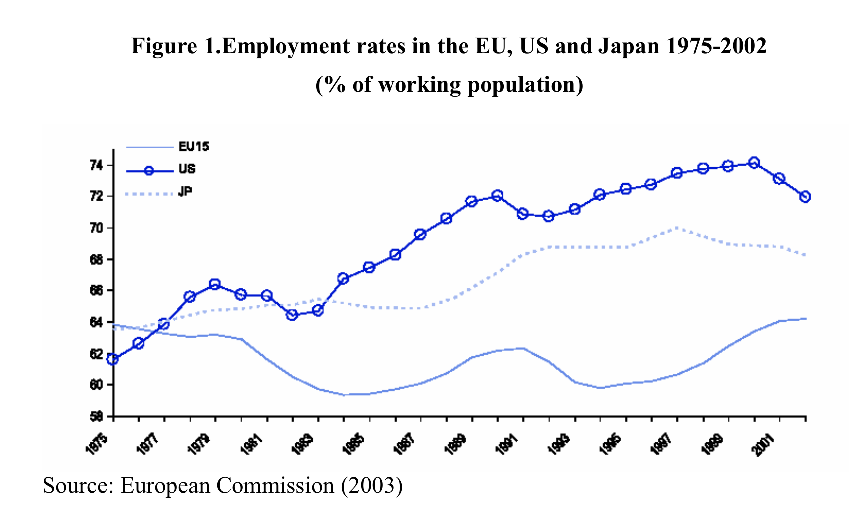
\includegraphics[scale=.7]{employment_rate}
  \end{figure}
\end{frame}


%--------------------------------------
\begin{frame}
  \begin{figure}
    \includegraphics[scale=.3]{first_enlargement.png}
  \end{figure}
\end{frame}

%--------------------------------------
\begin{frame}
  \begin{figure}
    \includegraphics[scale=.3]{second_enlargement.png}
  \end{figure}
\end{frame}

%--------------------------------------
\begin{frame}
  \begin{figure}
    \includegraphics[scale=.3]{third_enlargement.png}
  \end{figure}
\end{frame}

%--------------------------------------
\begin{frame}
  \begin{figure}
    \includegraphics[scale=.3]{fourth_enlargement.png}
  \end{figure}
\end{frame}

%--------------------------------------
\begin{frame}
  \begin{figure}
    \includegraphics[scale=.7]{mcquinn_whelan}
  \end{figure}
\end{frame}

%--------------------------------------
\begin{frame}
  \begin{figure}
    \includegraphics[scale=.7]{mcquinn_whelan2}
  \end{figure}
\end{frame}

%--------------------------------------
\begin{frame}
  \begin{figure}
    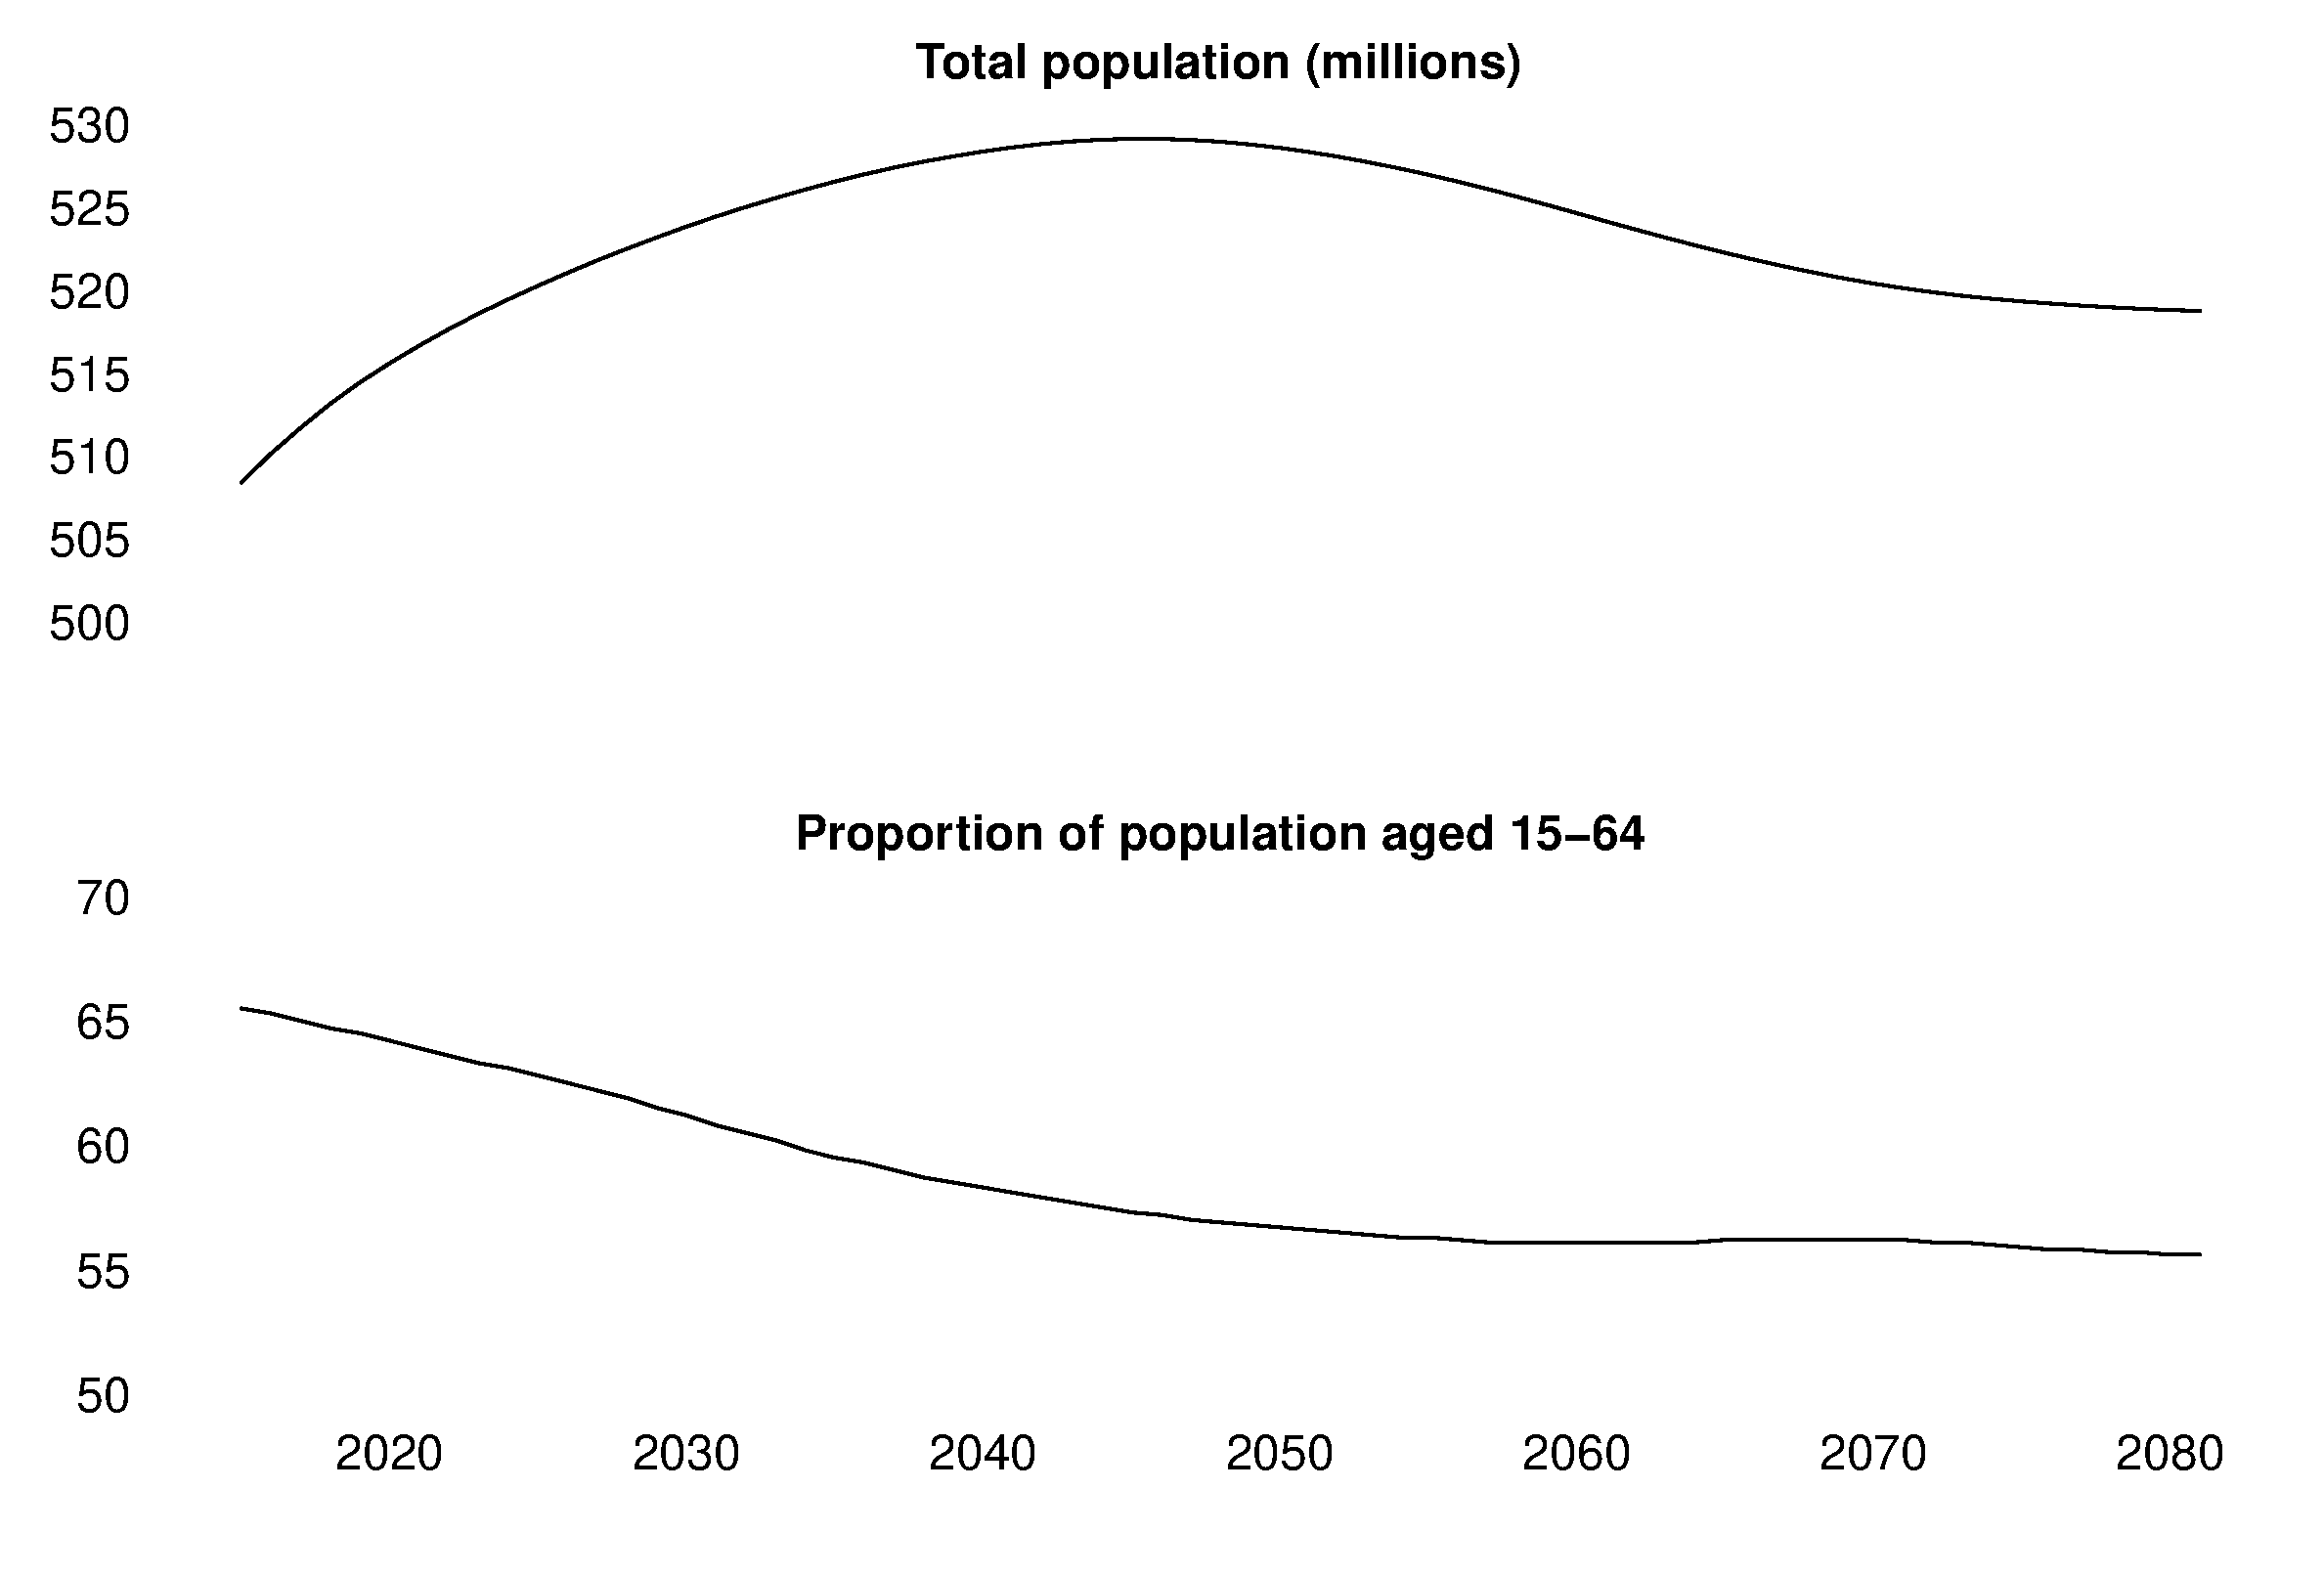
\includegraphics[scale=.3]{population}
  \end{figure}
\end{frame}

%--------------------------------------
\begin{frame}
  \begin{figure}
    \includegraphics[scale=.3]{new_member_states.png}
  \end{figure}
\end{frame}

%--------------------------------------
\begin{frame}
  \begin{figure}
    \includegraphics[scale=.25]{gdp_per_capita2}
  \end{figure}
\end{frame}


%------------------------------------------------------------------------------
\end{document}
